\chapter{Literature Review}
\label{ch-literature}


% Structure of ``Literature Review'':
% - Types of energy storage
% - Control of energy storage and its applications
%   - Open-loop and closed-loop control
%   - Distributed control
% - Gaps in literature
% - Summary

\section{Overview}
\label{ch-literature:sec:overview}

With the ongoing electrification and decarbonisation of the heat and transport sector, demand across the electricity network is expected to double by 2050 \cite{Wilks2010}.
One contributor towards this increasing demand is the expected uptake of LCTs as they start to penetrate power distribution networks.
Also, this uptake of LCTs is expected to not progress evenly throughout the network; instead clusters of early adopters are predicted to form \cite{Poghosyan2014}.
Such a scenario will result in LV networks to exceed their operational constraints even whilst the rate of LCT adaptation is at a relatively low national rate \cite{Poghosyan2014}.
Conventional reinforcement to extend the network's capacity is effective but expensive.
Together with recent availability of load information, due to the distribution and installation of smart-meters, the opportunity arises for DNOs to develop energy storage control strategies in order to achieve the greatest performance and add most benefits to their distribution networks.

In fact, according to the Department of Energy's global energy storage database, there are more than 1200 energy storage projects worldwide.
In the UK, as of 2016, 27 of those are installed and accumulate to an energy storage capacity of 33GWh \cite{Garton2016}.
Out of all global energy storage projects, 61\% use ``electro-chemical energy storage technology'', i.e. rechargeable batteries, and 49\% of those Battery Energy Storage Systems (BESS) are rated at less than 250kW.
Their sizes and ratings make such BESS suitable for deployment in distribution networks, and the figures in the energy storage database indicate that 131 of these projects are indeed used for LV network support \cite{DOE-GESD}.

A general survey of different roles for energy storage have already been presented in Section \ref{ch-introduction:subsec:role-of-energy-storage-a-survey}.
However, to align with the focus of this thesis on improving UK power distribution networks, Chapter \ref{ch-literature} will provide an extensive review on BESS applications and projects that support LV network operation; i.e. projects concerning voltage control mechanisms and power flow management.
The structure of this chapter is as follows.
First, in Section \ref{ch-literature:sec:topology-of-lv-network}, an overview of the UK power distribution network is given.
Then, the literature regarding energy storage projects and their applications in LV networks is reviewed in Section \ref{ch-literature:sec:energy-storage}.
Afterwards, in Section \ref{ch-literature:sec:control-of-energy-storage}, diffrent control approaches for energy storage are reviewed and compared.
In the end, in Section \ref{ch-literature:sec:literature-gaps}, the gaps are identified to highlight the research contribution and support the problem statement of this thesis.


\section{Role of energy storage - a survey}
\label{ch-literature:sec:role-of-energy-storage-a-survey}


\begin{figure}\centering
	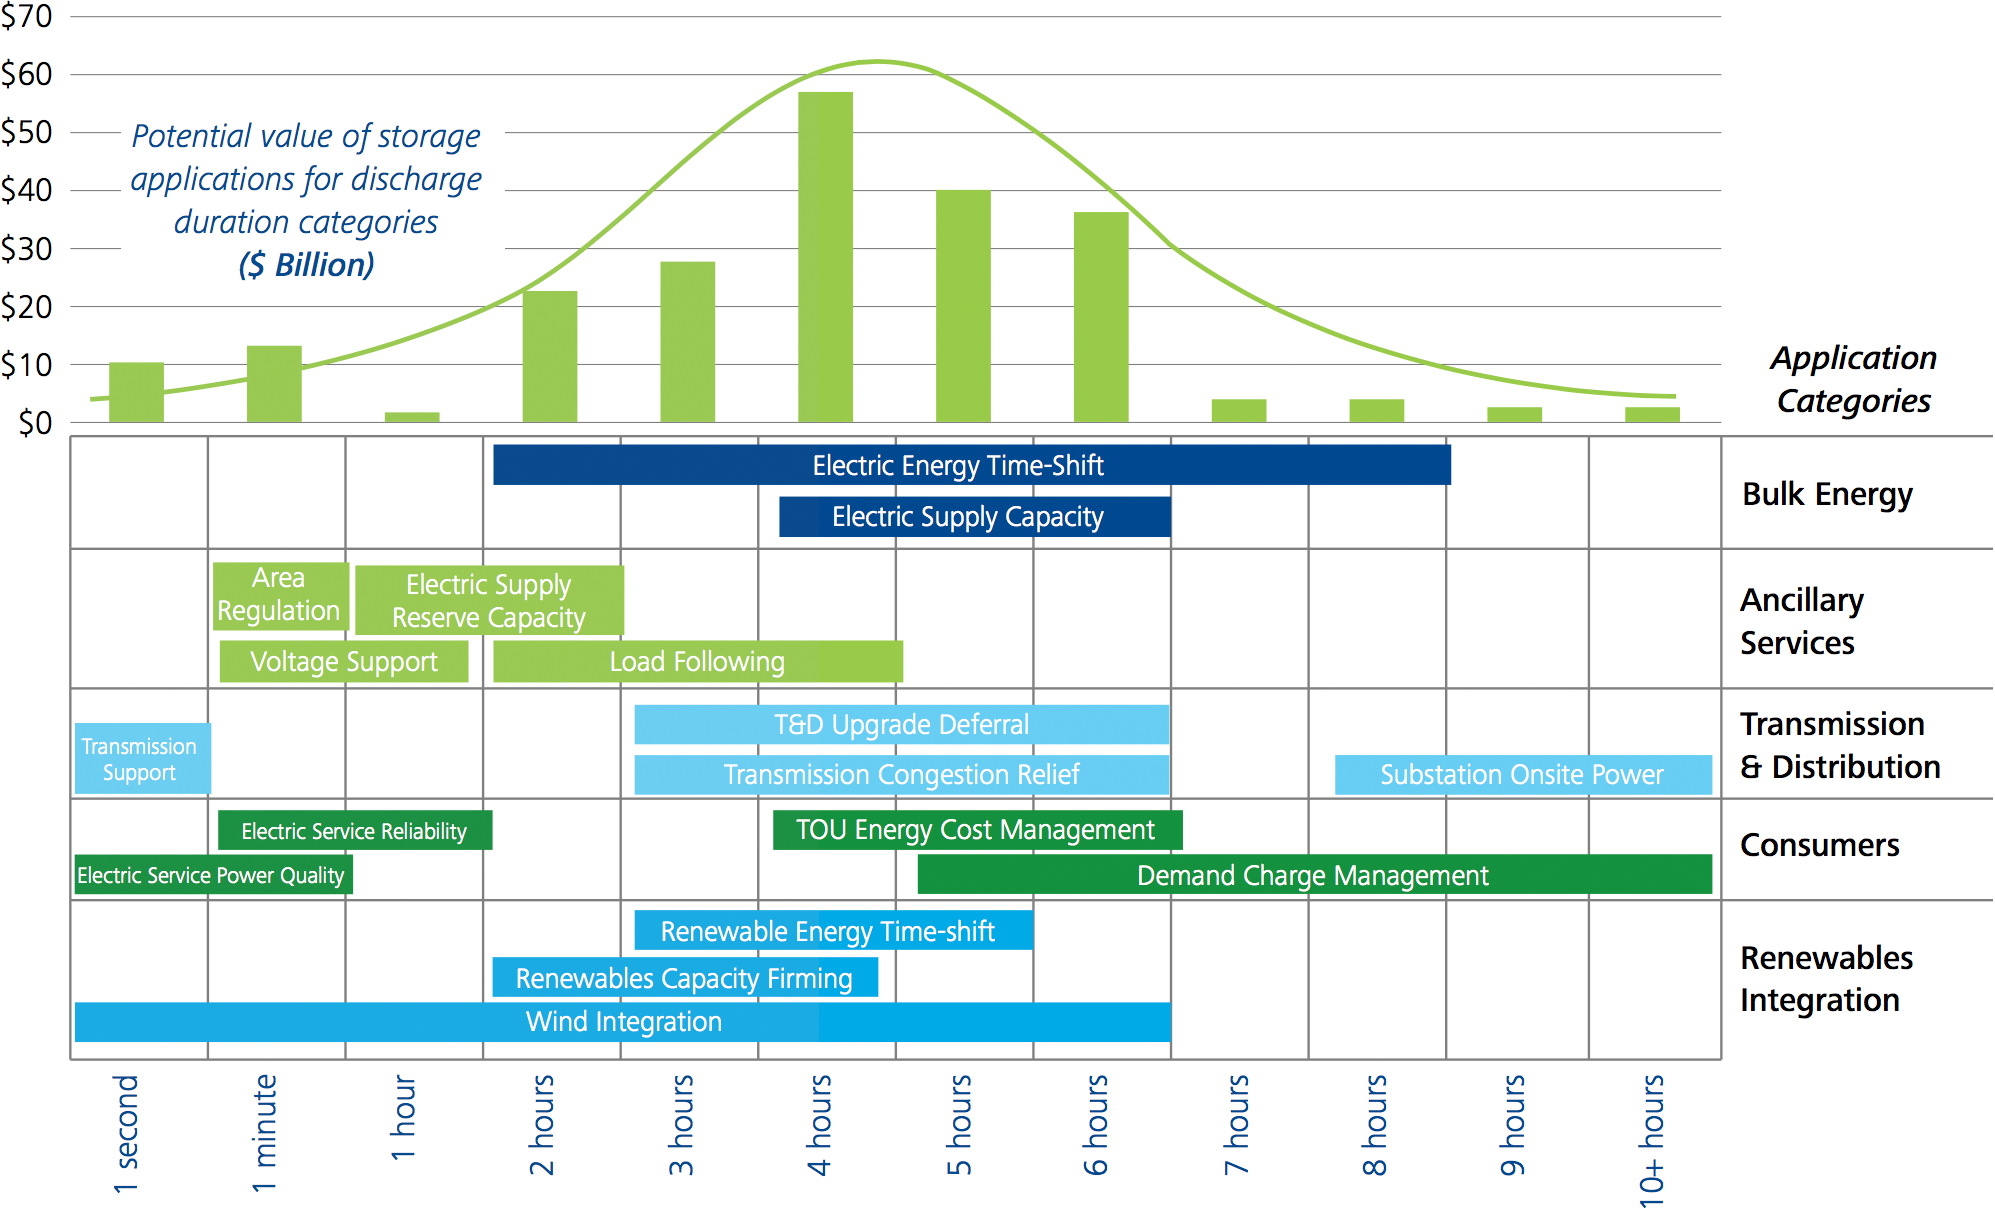
\includegraphics[width=\textwidth]{_introduction/fig/storage-financial-benefits}
	\caption{Energy storage applications and corresponding value for various discharge durations \cite{Deloitte2016}}
	\label{ch-introduction:fig:storage-financial-benefits}
\end{figure}

The idea of using energy storage in the electricity grid has been discussed for quite some time, and its important role in future energy systems has already been identified in the 70s \cite{Kalhammer1979}.
As the name suggests, electrical energy storage systems have the ability to both consume, store, and release electrical energy by converting it into a different form of energy.
Depending on the rate at which energy can be consumed and released, i.e. the system's power, as well as the amount of energy that can be stored, i.e. system's capacity, different functions can be provided.
A study for the Department Of Energy (DOE) showed that, when correctly exploited, these functions can yield direct financial benefits of \$157.56 billion over an estimated 10 year system lifecycle \cite{Eyer2010a}.
Figure \ref{ch-introduction:fig:storage-financial-benefits} shows these benefits in relation to their typical discharge period, and links them to their associated functions, too.
Here, Time Of Use (TOU) energy cost management yields the largest economic profit, yet from a historical point of view, bulk energy storage has played the most important role in the energy system.

Nowadays, storage can also tap into emerging revenue streams and perform additional functions.
As identified in several review articles \cite{Chen2009, Katsanevakis2017, Guney2017}, the key roles and applications of energy storage systems, regardless of profitability in the current market situation, can be identified as follows:

\textbf{Energy shifting - arbitrage}: This function uses the difference in energy price to yield revenue.
More specifically, as energy pricing is expected to become more dynamic and responsive to current energy demand and generation, storage is controlled to charge when energy prices are low and discharge when energy prices are high \cite{Chen2009, Leou2012}.
Such dynamic pricing schemes are expected to emerge due to significant changes in demand at morning and evening peaks \cite{Koohi-Kamali2013}.

\textbf{Supply capacity}: In order to meet future energy demand, energy suppliers commit their resources in advance.
Doing so allows them to plan for their operation and solve the economic dispatch problem.
With increasing demand, the supply volume will have to increase, too.
However, it is predicted that energy storage can defer or even avoid investments in power plants, assuming they are sized accrodingly (i.e. several 100MW)\cite{Dobie1998}.
Bulk energy storage was the first choice to support supply capacity.
One example is pumped hydro-electric energy storage, which has seen a global growth of 127GW since 1979 \cite{Rehman2015, Barbour2015, Barbour2016}.

\textbf{Ancillary services}: These services are of interest to transmission and distribution system operators since they support the operation of their networks.
For example, load following and frequency regulation are two complementing applications of that address the imbalance between demand and supply \cite{Bevrani2011}.
In case of a severe imbalance that resulted in network outage, black start is also a function that can be supplied by energy storage \cite{Cole1995, Kashem2007}.
Since modern energy storage systems can absorb and inject both active and reactive power, they can also provide voltage support \cite{Kulkarni2005}.

\textbf{Grid stability}: To make the grid more resilient to network faults (e.g. short-circuit or loss of a large generator), or to overcome scheduled network outages, energy storage can be used as an intermittent energy source \cite{Kundur1993}.
To provide optimal operation conditions for energy generators, storage can support rotor angle stability and voltage stability by injecting active and reactive power at the point of common coupling \cite{Chakraborty2012, Kolluri2002}.
Furthermore, sub-synchronous resonance and harmonic interference can also be reduced \cite{Wang1994}.
This coupling resonance can occur between electrical and mechanical systems and can damage the mechanical structure due to repetitive stresses and strains.

\textbf{Upgrade deferral}: As already stated in Section \ref{ch-introduction:subsec:solutions-to-mitigate-impact-of-lct}, both transmission and distribution systems would have to be upgraded unless energy storage could provide network-support functions.
By deferring network upgrades, network assets will be used more efficiently, and customer disruptions will be avoided \cite{Sayer2007, Eyer2010a}.
Furthermore, in areas where the expected load has already been met and growth has levelled out, deployed energy storage is flexible enough to provide alternative functions (unlike other network assets) \cite{Huff2013}.

\textbf{Transmission charges}: In scenarios where generators are charged to use transmission systems (due to the capacity limitations of the transmission system), energy storage could take advantage of the price structure to maximise the profit from the generated energy \cite{Sayer2007, Leou2012}.

\textbf{Congestion relief}: High congestion at substations of heavily loaded transmission or distribution lines can be tackled by co-located energy storage units \cite{Saez-de-Ibarra2013a, Kulkarni2005}.
This can be achieved by e.g. shaving peak load or relaxing the energy requirements from distributed generation \cite{Reihani2016, Gerards2016d}.

\textbf{Service reliability}: In areas where a string grid connection is required to assure e.g. industry operations, an ``uninterruptible power supply'' may be required.
Traditionally, these power supplies were diesel backup generators, but modern energy storage technology can provide similar services at lower cost \cite{Schoenung2001} (particularly when including alternative revenue streams).

\textbf{Power quality}: Sub-cycle and harmonic distortions on can severely deteriorate power quality, since they can have unwanted effects on connected equipment (similar to the issue of sub-synchronous resonance at the generation side).
Energy storage with modern power electronics could be capable of providing power filtering functions that suppress those distortion \cite{Putrus2007}.
This feature could be of particular interest to LV networks in the UK, since customers are arbitrarily connected to a single phase of a three-phase network.
Therefore, the discrepancy of power quality between the phases is even larger, yet available energy storage resources could even address this issue \cite{Miret2009} (especially when considering household connected units).


\textbf{Time-of-use energy charges}: A hurdle to DSM through flexible tariffs or TOU tariffs is the reason that consumers would have to adjust their energy consumption based on external price signals, which many are do not want to do.
Energy storage could however decouple the consumer form these tariffs and allow them to continue with their normal lifestyle \cite{Khani2014}.
Additionally, when exploiting the energy price difference, storage could even supply arbitrage functions to some customers and reduce their electricity bill \cite{Nair2010a}.
For customers with local generation, e.g. PV installation, their bill can be reduction even further.
This would be done by storing the generated energy until a period of high energy prices arises.
At this time energy storage could release the energy to maximise self-consumption \cite{Luthander2016}.

\textbf{Demand charges}: Larger customers, i.e. industrial and commercial loads, are not only charged for their total energy demand, but also their for their largest continuous power demand \cite{Oudalov2007, Mackey2013}.
Therefore, a factory that may use a relatively small amount of energy over a comparatively short amount of time, is billed accordingly.
After all, the infrastructure to deliver the required power needs to be installed and maintained.
In this scenario, energy storage could reduce the intermittent power demand without significantly increasing the total energy demand, and therefore reduce demand charges for larger customers \cite{Aghaei2013}.

\textbf{Renewables integration}: Unlike traditional energy sources, renewables have are highly volatile and have limited availability.
Since their availability, i.e. for solar PV, may not align with periods of high demand, i.e. during morning and evening, arbitrage functions may be provided to maximise the use of renewable generation - i.e. renewables ``shifting'' \cite{Zakeri2015}.
Furthermore, by discharging energy storage during times of low renewable generation, e.g. due to cloud cover or varying wind \cite{Jewell1987}, a continuous supply of energy can be assured - i.e. renewables ``smoothing''.
And lastly, if a renewable resource was committed for longer periods of time, yet the associated energy forecasts overestimated its generation capacity, storage can supply the gap to avoid balancing charges - i.e. renewables ``firming'' \cite{Chakraborty2012}.



\section{Energy storage projects in LV application}
\label{ch-literature:sec:energy-storage}

The challenge for DNOs to manage their distribution networks is caused by the DER's and LCT's difficult predictability, their volatile nature, and the weakness of the network into which they are deployed \cite{Woyte2006, Mohd2008a, Koureoumpezis2010, Bravo2015}.
Improved network management methods that are summarised under the term ``smart grid'' have thus become increasingly popular to counteract the negative impact from DERs (e.g. roof-top solar PV) and LCTs (e.g. EVs) \cite{Panteli2015}.
When however deferring the reinforcement or retrofitting of network assets to construct such a smart grid, deployment of BESS can provide a significant contribution to the integration of DERs and LCTs \cite{Grillo2012, Rowe2014a, Li2016, Hosseina2016a}.
As a result, DNOs have begun trialling of BESS across their distribution network to better their understanding and potential contribution \cite{NTVV2016, Lyons2015a, Ferreira2013a}.
%For the scope of reviewing BESS projects and applications in the LV network, both stationary and mobile BESS, i.e. vehicle-to-grid (V2G) enabled EVs, are considered.
To meet statutory and physical restrictions, voltage control and the power flow problem are two identified key challenges.

%\subsection{Voltage control}

\nomenclature[G]{OLTC}{On-Line Tap-Changer}

As already mentioned in Section \ref{ch-literature:sec:topology-of-lv-network}, UK distribution networks operate at 230V and have a statutory tolerance band of +10\% and -6\%.
Due to the varying load on the network, these voltages can deviate significantly.
Although todays deviation may not exceed the high-voltage or low-voltage thresholds, conduction losses and imperfect network conditions result in a lower overall system efficiency.
Traditionally, On-Line Tap-Changers (OLTC) are used to raise and lower voltages across the entire network to counteract such voltage deviations \cite{Sun2009}.
However, such a hierarchical voltage control with OLTCs has its limited applicability, especially in cases where the voltage deviation significantly differs for several branches of a feeding network \cite{Zangs2016}.
Installing a BESS at a strategic location, i.e. closer to the regions where voltage deviation takes place, and controlling the device to best suit the network's requirements is generally applicable and the commercially more viable alternative \cite{Liserre2010}.

As stated by Wade et al. \cite{Wade2009, Wade2010}, allocation of the BESS's limited storage capacity so it can solve the voltage problem most effectively is still a sophisticated challenge.
Nonetheless, by installing a 200kWh unit that is rated at 600kW in a project that was carried out with \textit{EDF Energy}, they showed the potential of BESS in a network to provide targeted voltage support.
Their results indicate a reduced voltage variation by 2.4\% and a complete elimination of any ``out-of-limit'' voltage events.
A demonstration project in Germany that was titled ``More Microgrids'' used four 180kWh batteries and demonstrated how both voltage stability as well as grid independence could be improved \cite{Overbeeke2010}.
In this project a collection of holiday homes were fitted with a distributed PV system that is capable of generating a peak power of 315kW, and BESS was used to maximise the utility from this generation.
However, due to the relatively small size of the network, due to the different behavioural patterns of holiday home occupants, and due to the different means of connecting customers to the German three-phase network, voltage deviation and phase unbalance issues were less dominant than they would be on a UK distribution feeder.
An equally sized project entitled ``GROWDERS'' also used multiple BESS in the LV network, but instead of focusing at grid independent network operation, they mainly contributed to frequency and thermal constraints as well as voltage stability \cite{GROWDERS2011}.

BESS that are sized between 100kWh to 200kWh (as those in the aforementioned projects \cite{Wade2010, Wade2009, Overbeeke2010, GROWDERS2011}) can easily address network, especially even when operating in a grid independent or ``islanded'' mode.
Results from these early field trials show how BESS store the excess renewable power for usage during later times.
But once capacity limits were reached, neither high or low voltage events could be omitted.
Such a result does indicate that not only the sizing, but also the BESS control method is of significant importance.

%\subsection{Power flow management}

Nonetheless, voltage violations that require strong voltage support have not yet been encountered in any of these projects.
In fact, the majority of low-voltage events on the UK distribution networks, i.e. when voltage levels fall below 216.2V, are caused by anomalous network events or failures of the measurement equipment \cite{UKPowerNetworks2014a}.
Therefore, the complementing task of choosing correct control methods to optimally manage the network's power flow is also important.
This is partly due to measurement equipment in LV substations being more reliable and precise than traditional smart meter readings, but also since it is excessive power flow that causes operational issues which do eventually lead to system overloads and outages \footnote{%
In fact, according to the UK energy regulator \textit{OFGEM}, on average 45\% of all customers experienced service disruptions in the period 2015-16 \cite{Ofgem2017}.
Whilst unanticipated outages due to severe winter weather did lead to \pounds39 million worth of damages, network upgrades to prevent outages and repairs after outages had happened, did however contributed the larger amount of customer interruptions and customer minutes lost \cite{Ofgem2014}.%
}\cite{Putrus2009, Pillai2010}.
To prevent future power flow from exceeding the system's capacity, BESS has been proposed to function as an instantaneous reserve \cite{Kunisch1986a, Kunisch1986}.
The resulting droop control method uses local voltage and frequency measurements to infer the latest loading and stress on the network to issue corresponding BESS control instructions \cite{Engler2005a}.
Droop control is founded on the assumption that network frequency will drop as demand begins to exceed supply, and that voltages along the distribution feeder drop more significantly when load is increased.
Yet as already stated in Section \ref{ch-literature:sec:topology-of-lv-network}, reversed power flow raises voltage levels, which makes such control methods a less reliable source of network stress information.
This problem was also encountered by Riffonneau et al. in \cite{Riffonneau2011}, where they control BESS to solve an optimal power flow problem for grid connected PV systems.
Ultimately, they were able to achieve 13\% gain on electricity bills by implementing a rule-based dynamic programming optimiser, and they reduced peak power by successfully integrating PV.
However, they do not consider reactive power within their power management method, although it could free additional network resources and yield  yield benefits to the distribution network.
The reason behind excluding it form their study was due to the potential conflicts that may arise with the proposed voltage control method, which heavily relies on voltage measurements.
Using BESS to reallocate PV generation for maximised self-consumption \cite{SaniHassan2017} or to achieve ``peak-shaving'' behaviour \cite{Bennett2015, DePaola2016} has seen continued interest in the field of BESS power flow management.

Aiming to address both voltage and power flow problems, \textit{Scottish and Southern Electricity Networks} (SSEN) became the first UK network operator to trial street-level BESS deployment in the LV network, and they installed 500kWh worth of storage in Bracknell, UK \cite{SSEN2016}.
This capacity was achieved by 25 Energy Storage Management Units (ESMUs) that each had cascadable 12.5kWh Energy Storage Units (ESUs).
These ESUs were connected to the distribution network via a three-phase 36kW Power Electronic Units (PEUs) to both manage the batteries and perform filtering operations.
The aim of this so called \textit{New Thames Valley Vision} (NTVV) project was to understand potential benefits, practicalities and costs of installing street-level BESS.
In the beginning, the main problem of finding an optimal deployment location for the ESMUs, to achieve their best possible impact on system voltages had to be addressed.
Yunusov et al. and Rowe et al. in \cite{Yunusov2016, Rowe2014, Rowe2014a} worked in collaboration with \textit{SSEN}, and they assessed different BESS locations in several networks.
They found that a location 4/7 to 2/3 down the feeder yields the best overall impact on voltage levels.
However, their findings also show that this location can vary significantly when not only focusing on voltage support; i.e. proximity to the feeding substation was of greater importance when reducing the system's overloads or distribution losses.
The considered BESS control methods and those implemented in the NTVV project are reviewed in the next section, Section \ref{ch-literature:sec:control-of-energy-storage}.










\section{Control of energy storage and its applications}
\label{ch-literature:sec:control-of-energy-storage}

Installing BESS at a strategic location in the LV network brings several advantages to DNOs' control over the network's performance.
Regulating voltages to stay within statutory operating bands \cite{Yang2014}, improving power quality by optimising its power factor \cite{Chua2012b}, shaving peak load to relieve stress from the installed network assets \cite{Bennett2015} or reducing phase unbalance to increase network efficiency \cite{Wang2015b} are only a few examples of recent research in this field.
Whilst the questions regarding locating and scaling of BESS have mostly been addressed, BESS control still remains an open question and can be split into two complementing yet unmarried approaches:

\begin{enumerate}
	\item ``off-line'' control, using load forecasts and BESS schedules; and
	\item ``on-line'' control, using Set-Points Control (SPC), Model Predictive Control (MPC) or similar dynamic control methods.
\end{enumerate}

These two control approaches have evolved from two different fields of active network management.
Nonetheless, both approaches hold significant benefits to the operational performance of power distribution networks and neither of the two can be neglected.
Therefore, Section~\ref{ch-literature:subsec:off-line-and-on-line-control} addresses and discusses the two control approaches and their missing link.

The current form of the NTVV project focuses on controlling a single BESS in the LV distribution network.
However, the uptake of household connected BESS will increase the number of distributed systems, which need to be managed cooperatively.
Therefore, Section~\ref{ch-literature:subsec:centralised-and-distributed-control} reviews and discusses different control approaches for distributed BESS since the control of multiple single-phase storage units in a three-phase network is inherently more challenging that controlling one three-phase device.

\subsection{Off-line and on-line control}
\label{ch-literature:subsec:off-line-and-on-line-control}

Off-line control uses historic data to predict future load patterns which are used to schedule BESS operation accordingly.
Early approaches by Oudalov et al. \cite{Oudalov2007}, who used dynamic programming to generate BESS schedules had relatively high forecast errors due to the inherent difficulty of predicting future loads.
These errors ultimately limit the ability of any given BESS schedule to effectively reduce peaks.
This is why recent research begun including uncertainty, like the work done by Baker et al. \cite{Baker2017} where uncertainty of wind power was taken into account when scheduling and sizing BESS.
Other work frequently re-evaluates BESS schedules to control and adjust its schedules after completing individual decision epochs \cite{Wang2014a}.
Nonetheless, load forecasting remains a key component for BESS scheduling despite those load forecasts (and the resulting BESS schedules) being imperfect.
This fact was emphasised by Rowe et al. in \cite{Rowe2014a}, and they developed a filtering mechanism for scheduling algorithms to reduce peak load in LV networks due to the presence of forecast errors.
They also highlight the fact that most day-ahead load forecasts only predict at a temporal resolution down to half-hourly periods which makes estimating errors at higher temporal resolution less dominant.
The reason behind choosing this half-hourly forecasting period was pointed out by Haben et al. in \cite{Poghosyan2014, Haben2014}, as they argue that forecasts at half-hourly resolution yield the best compromise between high accuracy and high temporal resolution.
Therefore, half-hourly forecasts have become the standard for generating any resource commitment and resource operation schedules.
However, sub-half-hourly load volatility imposes the biggest stress on the network and it is this volatility that cannot be addressed when relying on half-hourly forecast alone.
In conclusion, on-line control has been considered as an alternative to off-line control.

One flavour of on-line control is the Set-Point Control (SPC) which is a robust technique that can immediately respond to network changes.
SPC achieves this behaviour by measuring some properties of the power system (for example voltage level or frequency) and comparing those values to an internal target value, i.e. the set-point.
Droop control, as mentioned in Section~\ref{ch-literature:subsec:power-flow-management}, was one of the first control methods that followed the SPC paradigm.
A single set-point is however not suitable for a network that changes dynamically which is why droop control was extended to become adaptive as done by Tayab et al. in \cite{Tayab2017}.
Their research shows how conventional droop control runs the risk of allowing system frequency to drop to 48.4Hz (from a nominal 50Hz), whereas adaptive droop was capable of frequency restoration with little to no observable frequency variation.
However, their solution relied on PV and gas turbines to provide active power injection and could only injected reactive power into the system when these are not available - a comparable scenario may occur when BESS completely discharges.
Therefore, voltage compensation may still be realised, but frequency remains unchanged.
Conventional droop control does therefore run the risk of reaching energy shortage or surplus if the set-points and system dynamics are chosen too low or high.
Modifications like hysteresis control and ramp-rate control were proposed to yield an adaptive SPC \cite{Blaabjerg2006, Malesani1990, Xu2011a, Such2012}.
Hysteresis control prevents the device from oscillating between different power states even when small changes in the network are detected and would otherwise trigger an SPC change.
When implementing a dead-band around the controller's set-point as well as utilising a ramp-rate control, as done by Such et al. in \cite{Such2012}, BESS can correct its internal energy state and therefore prevent hitting its operational limits.
Furthermore, Such et al. showed how reverse power flow can be completely omitted through the use of on-line BESS control.
However, this kind of on-line control is less effective when addressing daily demand peaks since pure SPC can only react to present network demand and does not respond to general trends or upcoming load events.

In order to address these shortcomings SPC has been extended by using short-term load predictions through the implementation of Model Predictive Control (MPC) \cite{Gybel2012, Hatziargyriou2015}.
Some MPC examples include Auto-Regressive (AR) models \cite{Li2009, Nie2011}, fuzzy logic models \cite{Sannomiya2001, Chen2013a}, genetic algorithms \cite{Xia2015a, Liu2015} or Artificial Neural Networks (ANN) \cite{Kalogirou2014, Quan2014, Lee2014, Pezeshki2014, Vaz2016, Reihani2016, Xiao2017}.
Advancements in computational power allowed ANN to gain traction, and as shown in the study by Quan et al. in \cite{Quan2014} ANN is becoming a promising method to generate load forecasts.
In fact, in their study, Quan et al. proved how ANN can outperform AR and fuzzy logic models given that the ANN was optimally trained.
Therefore, MPC can yield a acceptable prediction performance for linear systems when its complexity is sufficiently increased.
For instance, Reihani et al. in \cite{Reihani2016} used the most recent 20 minutes of load information with a complex-valued ANN to predict the next 20 minutes of minutely load variations.
Since their raw forecasts were more erratic than the actual load profile, a Kalman filter was implemented to smoothen the MPC's output, yet this step introduced significant discrepancies between the actual and the forecasted load.
Therefore they increased MPC complexity even further by taking into account parallel time-series, i.e. they considered the same 20 minutes from previous days in the prediction mechanism.
This addition produced significantly better results and they shaved daily peaks by around 300kW (from 1.6MW) in the medium-voltage network.
Implementing such increasingly complex MPC to support on-line control is therefore a promising research trend, however the computational burden to deliver real-time solutions makes deployment of such systems costly and/or difficult.

Therefore, finding a way of combining both off-line control (i.e. scheduled BESS operation which is executed at half-hourly resolution) with on-line control (i.e. a mechanism that is responsive to power system changes) allows application of real-time corrections to the BESS schedule.
Since this is still an open and ongoing research problem that has not yet been solved, \ref{objective-1} and \ref{objective-2}, as outlined in Section~\ref{ch-introduction:sec:problem-statement}, aim to develop and present a control mechanism that utilises the benefits from scheduled and real-time control.
The objectives' corresponding chapters are, respectively, Chapter~\ref{ch1} and Chapter~\ref{ch2}, and they address this research problem in two stages.
At first the problem is addressed by developing a framework to apply scheduled BESS operation to a three-phase network in a sub-half-hourly manner but without modifying its underlying half-hourly schedule.
Secondly, this hard constraint is removed by developing and implementing a dynamic controller that allows an operational tolerance around the pre-computed BESS schedule in order to guide BESS operation without violating its energy storage limits whilst maximising its flexibility to respond to sudden system changes.
This a control system does however rely on a communication infrastructure in order to be implemented and deployed in reality.
These infrastructures and their underlying control either follow a centralised or distributed networking paradigm.
Both paradigms entail their specific costs and benefits which are addressed in the subsequent section, Section~\ref{ch-literature:subsec:centralised-and-distributed-control}.

\subsection{Centralised and distributed control}
\label{ch-literature:subsec:centralised-and-distributed-control}

It is important to understand the topology of an on-line control system since most of them have to gather power system information from multiple locations in order to make intelligent control decisions.
This is particularly true if the control system consists of multiple entities that are distributed across the power network.
The monitoring and control of such a distributed system (and hence of any power network) includes four systems that are inherently linked \cite{Mansouri-Samani1993}:

\begin{enumerate}
	\item The \textit{managed system} itself, like a power network, that needs to be controlled;
	\item a \textit{monitoring system} that generates data through sensors and measuring equipment that is installed in the \textit{managed system};
	\item a \textit{decision making system} that uses the provided data to generate certain aims, to improve the system state; and
	\item a \textit{control system} to generate control actions for the \textit{managed system}.
\end{enumerate}

\nomenclature[G]{IoT}{Internet of Things}
\nomenclature[G]{SCADA}{Supervisory Control And Data Acquisition}

In traditional power system control, systems 1 and 2 are grouped into the distributed measuring system and systems 3 and 4 are grouped into a centralised controller \cite{Nelson1985}.
Therefore a bidirectional flow of information must exist in order to control and assure operation of the underlying physical network.
Supervisory Control And Data Acquisition (SCADA) is the typical control architecture that enables the implementation of this bidirectional information flow.
Tokyo is a showcase of successfully implementing such a centralised control system on a very large scale.
In 1990, \textit{Tokyo Electric Power Co.} (TEPCO) and \textit{Toshiba} presented their latest installation of a centrally managed power distribution network that could deliver 43GW of power to the entire city of Tokyo \cite{Matsuzawa1990}.
All control instructions were generated from TEPCO's central dispatching centre, which took into account measurements from a network of 819 nodes and 938 branches.
Since Tokyo has grown significantly over the past decades, computational burden to relay data and act upon the information has increased, too.
The UK transmission system is also a centrally managed system that has seen an increase in complexity, yet in 2017 ``\textit{the network is 99.9999\% reliable - a statistic we're proud of}``\cite{NationalGrid2017}.

\nomenclature[G]{FIPA}{Foundation for Intelligent Physical Agents}
\nomenclature[G]{ICT}{Information and Communication Technology}

But with the deployment of smart meters, network enabled appliances and controllable LCTs that can be part of the so called ``Internet of Things'' (IoT) system complexity is expected to increase beyond the capabilities of a single central management centre.
This reason is why research began focusing on distributed control mechanisms \cite{Vovos2007, Guerrero2008, Bidram2014, Toledo2013, Marra2013, Gill2014, Dolan2012, Atia2016, Bidram2012, Wang2016}.
For example, Vovos et al. in \cite{Vovos2007} compared centralised and distributed systems for voltage control and showed how they can yield a 86\% gain (using centralised control) and 72\% gain (using distributed control) in connectible capacity.
Adding distributed BESS into the energy mix, Toledo et al. in \cite{Toledo2013} evaluated its impact on the IEEE-14 bus network when subjected to PV energy injection.
Their developed voltage index showed how voltages can deviate from nominal levels.
In their results this index was 0.074\%, 2.823\%, and 3.471\% for a release of system capacity of 500kW, 1000kW, and 1500kW, respectively.
In their work a higher index represents a larger voltage deviation in comparison to a predefined base case without PV or BESS.
To counteract this voltage rise, research like that by Marra et al. in \cite{Marra2013} used coordinated EV charging to maximise self-consumption and thus alleviate grid power injection by PV.
Focusing on the LV network's voltage issues, Marra et al. showed how high voltage incidents are completely avoided by charging at strategic times throughout the day, and at relatively low charging powers of 3.5kW.
In fact, the majority of existing literature that uses BESS in distribution networks focuses on voltage security \cite{Sugihara2013, Toledo2013, Marra2013, Mokhtari2013, Atia2016}, power flow management \cite{Guerrero2008, Wang2016} and management of flexible loads \cite{Gill2014, Dolan2012}.
For instance, the approach used by Mokhtari et al. in \cite{Mokhtari2013} relies on bus voltage and network load measurements to prevent system overloads, and Marra et al. in \cite{Marra2013} go even further and use information sharing between PV and BESS in order to limit voltage deviation.
Both research teams were able to stabilise the network, and Marras et al. even increased the voltage margin by an additional 6.1V.
The reasons why the usage of distributed and hierarchical control systems have become this attractive include lighter computational load for all control systems through abstraction at higher control levels and improved system stability, security and redundancy \cite{Guerrero2013, Guerrero2013a}.

Approaches and topologies to manage the flow of information within these control systems are classified by Bidram et al. in \cite{Bidram2014} where they separate the real network (i.e. the \textit{physical layer}) from Information and Communication Technology (ITC) (i.e. the \textit{cyber communication layer}).
This separation allowed them to represent any distributed power system as a system of multiple cooperating entities, i.e. intelligent agents that form a so called Multi-Agent System (MAS).
The technology of MAS comes from computer science and is well established in theory and practice of intelligent agents \cite{Russell2009}.
As stated by Wooldridge et al. in \cite{Wooldridge1995} intelligent agents are flexible and autonomous entities that are defined by three fundamental properties:

\begin{enumerate}
	\item \textit{Reactivity}, which allows an agent to respond to changes in its observed environment,
	\item \textit{Pro-activeness}, which makes an agent act to meet its own or a collaborative goal, and
	\item \textit{Social-ability}, which enables the agent to coordinate its action with other agents.
\end{enumerate}

Computer scientists would describe an agent as a component that gathers and collaboratively reacts to information about its environment.
But distributed control systems in power distribution networks share the same characteristics.
For this very reason MAS has seen increasing attention in the power and energy engineering disciplines.
Some MAS applications are focusing on integration of DERs \cite{Al-Hinai2004, Dimeas2005, Dou2017, Vasirani2013, Gomez-Sanz2014}, matching of demand and supply \cite{Kok2005}, restoring the power distribution network \cite{Li2012}, reconfiguring the network to reduce unbalance \cite{Ding2016}, integration of EVs \cite{Lopez2011, Karfopoulos2013, Ramachandran2013, GrauUnda2014} and providing voltage support \cite{Baran2007}.
For example, Dou et al. in \cite{Dou2017} proposed a MAS that coordinates DERs in as a so called Virtual Power Source (VPS).
This VPS is an aggregate of all distributed entities and responds to voltage events throughout the LV distribution systems.
In the case where generation increase would raise voltage levels beyond their statutory limits their VPS control could maximise power sharing and thus limit voltage overshoot to stay within voltage tolerance.
This VPS is typically referred to as a Virtual Power Plant (VPP), which has also been implemented as a MAS by Vasirani et al. in \cite{Vasirani2013}.
In their work Vasirani et al. propose a distributed control strategy that utilises EVs as an energy storage medium to maximise profits from operating distributed renewable energy sources.
Their findings suggest that when providing 12kWh of the EV's energy storage capacity for renewable integration an annual EV profit of more than \texteuro250 (at 40\% depth of discharge) can be achieved.
However, research involving MAS or any distributed control for that matter does require strong and standardised communication mechanisms.

A standard for MAS was established by the Foundation for Intelligent Physical Agents (FIPA) since the underlying versatility of different MAS would otherwise make integration very challenging.
This challenge was also raised by Catterson et al. in \cite{Catterson2005}, where they tried to merge the Condition Monitoring Multi-agent System (COMMAS) \cite{McArthur2004a} with the Protection Engineering Diagnostic Agents (PEDA) system \cite{Hossack2003a}.
They showed the inherent difficulty of combining different ontologies despite the similar underlying goals.
Also, as the number of independent elements becomes ubiquitous requirements for a strong telecommunication infrastructure become equally important \cite{Hatziargyriou2015}.
So far synchronisation amongst agents has been taken for granted, yet MAS on multilayer networks may not automatically be synchronised \cite{He2017}.
The impact of desynchronised information exchange on the performance of a MAS driven energy scheduling algorithm still remains an open research question.
Therefore, assessing the impact of introducing such a desynchronisation has become part of the research that is presented in this thesis, and \ref{objective-3} as outlined in Section~\ref{ch-introduction:sec:problem-statement} aims to answer this research question.
Regardless of the synchronised or desynchronised nature of the distributed control, they both do however require some kind of communication infrastructure which may not always be present.
Therefore, the next section, Section~\ref{ch-literature:subsec:communication-less-control}, introduces control mechanisms where communication between devices is no longer a strong requirement.

\subsection{Communication-less control}
\label{ch-literature:subsec:communication-less-control}

Lastly, developing control methods for distributed system that do not rely on a communication infrastructure is also an important research topic since this infrastructure may not always be available; despite this being a common assumption \cite{Hatziargyriou2015}.
So called communication-less systems are typically collections of multiple ``dumb'' devices that follow their own control instructions without any external inputs.
The current procedure of charging EVs is a perfect example of such a system since their charging typically commences immediately after they have been plugged into the grid.
At the current rate of EV uptake so called ``dumb charging'' (or any ``dumb action'' for that matter) has high potential of causing significant network issues \cite{Hota2014, Liu2015a}; i.e. voltage deviations, equipment overloads, asset damage and system outages.
This issue is amplified since the EV uptake is anticipated to increase as driving range increases, cost of purchase decreases and the emphasis on leading an environmentally-friendly lifestyle is favoured more \cite{Shah2015}.
ICT reliant distributed control methods aim to circumvent these issues by using Demand Side Management (DSM) strategies.
In \cite{Mohsenian-Rad2010} for example, Mohsenian-Rad et al. based developed a DSM mechanism that was based on game theory where multiple users engaged in the energy market to minimise the Peak-to-Average Ratio (PAR) of the resulting demand profile.
Their results show that both minimising financial cost or the PAR of the resulting demand profile resulted in a 21.9\% reduction in PAR when compared to a scenario without scheduling the energy consumer.
But minimising PAR resulted in only a 7.31\% reduction in energy cost, whilst minimising cost directly lead to a 19.6\% reduction, despite the similar improvements in demand profile.
However, this approach highly relies on ICT, as do similar DSM approaches that use for example time-of-use tariffs \cite{Deilami2011, Surles2012} or other pricing signals \cite{Masoum2015}.
None of them can be implemented without ICT and instead an indirect method must be sought.

\nomenclature[G]{AIMD}{Additive Increase Multiplicative Decrease}
\nomenclature[G]{V2G}{Vehicle to Grid}

A communication-less form of controlling Distributed Energy Resources (DERs) is the already mentioned Set-Point Control (SPC) \cite{Leadbetter2012}.
Using traditional SPC on multiple identically-configured DERs can provide an optimal operation conditions, if each DER's control parameters (bus voltage) were shared \cite{Thieblemont2017a}.
But in a communication-less environment this requirement cannot be satisfied which is why DER control algorithms have to be improved to prevent for example devices located furthest from the substation from being used more frequently than others.
The algorithm that is to be extended to control several BESS in a LV network is the Additive Increase Multiplicative Decrease (AIMD) algorithm.
Unlike traditional SPC or hysteresis control like in \cite{Jiang2007}, where a fuel-cell's bus voltage was used as input to a ramp control for active power sharing, AIMD (like MAS) has its roots in computer science.
Originally, AIMD algorithms were applied to congestion management in telecommunication networks using the TCP protocol \cite{Chiu1989} to maximise utilisation while ensuring a fair allocation of data throughput amongst a number of competing users \cite{Wirth2014}.
The same AIMD-type algorithms have previously been applied to power sharing scenarios in low voltage distribution networks where the limited resource is the availability of power throughput capacity of the substation's transformer.
One of the first proposed implementations for DER management was by St{\"{u}}dli et al. \cite{Studli2012}, yet their system still required a one-way communication infrastructure to broadcast a so called ``capacity event'' \cite{Studli2014, Studli2014a}.
Later their work was extended to include Vehicle to Grid (V2G) applications with reactive power support \cite {Studli2015}, but this work still relied on a functioning and robust ICT infrastructure.
Therefore, the question whether a truly communication-less dynamic control method can be developed (i.e. mitigating voltage deviation and capacity limitations) is still a remaining research problem.
More specifically, this control method should not only avoid to impose any ICT requirements, but it should also aim to equalise the utilisation of all controlled devices which is not guaranteed by the traditional AIMD algorithm.
\ref{objective-4}, as outlined in Section~\ref{ch-introduction:sec:problem-statement} aims to solve this research problem by extending AIMD to AIMD+, where natural voltage drops are taken into account to correctly skew the algorithm's control decisions for individual control entities.
Previous research is therefore extended since previous work has only utilised common SPC thresholds for controlling each of the DERs or previous work relied still on some form of communication infrastructure.
In strong contrast to the former objectives of this thesis where substation monitoring was used, the proposed AIMD+ algorithm does not require this information or any communication infrastructure for that matter.


\section{Summary of gaps in literature}
\label{ch-literature:sec:literature-gaps}

\hl{THIS SECTION SUMMARISES LITERATURE, ITS GAPS AND LINKS THEM TO OBJECTIVES}

The UK's electrification of the heat and transport sector, and its introduction of LCTs into the LV distribution network is expected to put significant strain onto the installed assets.
Through integration of distributed renewable generation the additional load is aimed to be reduced, however renewable volatility makes their integration a significant challenge.
To support the integration of DERs and LCTs by addressing operational constraints, i.e. voltage bands and thermal limits, BESS has been deployed.
Whilst research has already focused on sizing, locating and operating BESS, BESS operation can still be split into two unlinked categories: off-line control or forecast driven control and on-line control or Model Predictive Control (MPC).
Whereas off-line control takes into account daily load trends (i.e. at half-hourly resolution), it cannot compensate for load volatility due to DERs and LTCs (i.e. at sub-half-hourly resolution).
On-line control methods on the other hand are designed to react quickly when system changes occur (i.e. at sub-half-hourly resolution), but they cannot efficiently include daily or weekly load patterns (i.e. at half-hourly resolution) due to the increase in model complexity.
On the basis of the gaps in literature, as highlighted above, and the problem statement that is stated in Section \ref{ch-introduction:sec:problem-statement}, research objectives 1 and 2 have been derived.

Furthermore, as the number of distributed entities increases throughout the grid, methods to manage those entities need to become more sophisticated.
Yet when the system complexity exceeds the available computational resource, then centralised control cannot deliver real-time instructions.
As a result, control is being distributed using different implementations of MAS, e.g. Internet of Things (IoT) or Virtual Power Plant (VPP), where several intelligent agents collaborate to improve the network's operation.
However, all developed algorithms either explicitly or implicitly assume synchronisation amongst all control entities, which need not be the case in reality.
Assessing how information desynchronisation impacts the performance of a distributed algorithm is still an open research question.
ref{objective-3} and 4 as outlined in Section \ref{ch-introduction:sec:problem-statement} address this question by performing the assessment and developing an algorithm that no longer depends on communication systems.

To summarise, the problems that arises from the identified gaps in literature are:

\begin{itemize}
	\item how to assign pre-scheduled BESS powers to three-phase networks in order to yield the largest positive impact on the underlying network (\ref{objective-1}),
	\item how to adjust a half-hourly BESS schedule, which is based on a realistic and erroneous load forecast, based on sub-half-hourly power variations (\ref{objective-2}),
	\item how large the impact will be on the performance of a distributed control algorithm when information or message passing amongst the control entities becomes desynchronised (\ref{objective-3}), and
	\item how multiple BESS can be coordinated in a communication-less environment whilst contributing to voltage stability and thermal constraints without allocating their resources unevenly (\ref{objective-4}).
\end{itemize}

Despite some of the literature including aspects of the proposed research, none of them answer the research questions that are identified above.
The novelty of the research in this thesis consists of combining on-line and off-line control, as well as to assess and extend the control of distributed BESS.
All contributions and publications, as presented in Section \ref{ch-introduction:sec:contributions} and \ref{ch-introduction:sec:publications}, respectively, reflect upon the novelty of the presented research against the objectives and gaps in literature.


\section{Summary of Gaps in Litearture}
\label{ch-review:sec:summary}

%\section{Overview}
\label{ch-literature:sec:overview}

With the ongoing electrification and decarbonisation of the heat and transport sector, demand across the electricity network is expected to double by 2050 \cite{Wilks2010}.
One contributor towards this increasing demand is the expected uptake of LCTs as they start to penetrate power distribution networks.
Also, this uptake of LCTs is expected to not progress evenly throughout the network; instead clusters of early adopters are predicted to form \cite{Poghosyan2014}.
Such a scenario will result in LV networks to exceed their operational constraints even whilst the rate of LCT adaptation is at a relatively low national rate \cite{Poghosyan2014}.
Conventional reinforcement to extend the network's capacity is effective but expensive.
Together with recent availability of load information, due to the distribution and installation of smart-meters, the opportunity arises for DNOs to develop energy storage control strategies in order to achieve the greatest performance and add most benefits to their distribution networks.

In fact, according to the Department of Energy's global energy storage database, there are more than 1200 energy storage projects worldwide.
In the UK, as of 2016, 27 of those are installed and accumulate to an energy storage capacity of 33GWh \cite{Garton2016}.
Out of all global energy storage projects, 61\% use ``electro-chemical energy storage technology'', i.e. rechargeable batteries, and 49\% of those Battery Energy Storage Systems (BESS) are rated at less than 250kW.
Their sizes and ratings make such BESS suitable for deployment in distribution networks, and the figures in the energy storage database indicate that 131 of these projects are indeed used for LV network support \cite{DOE-GESD}.

A general survey of different roles for energy storage have already been presented in Section \ref{ch-introduction:subsec:role-of-energy-storage-a-survey}.
However, to align with the focus of this thesis on improving UK power distribution networks, Chapter \ref{ch-literature} will provide an extensive review on BESS applications and projects that support LV network operation; i.e. projects concerning voltage control mechanisms and power flow management.
The structure of this chapter is as follows.
First, in Section \ref{ch-literature:sec:topology-of-lv-network}, an overview of the UK power distribution network is given.
Then, the literature regarding energy storage projects and their applications in LV networks is reviewed in Section \ref{ch-literature:sec:energy-storage}.
Afterwards, in Section \ref{ch-literature:sec:control-of-energy-storage}, diffrent control approaches for energy storage are reviewed and compared.
In the end, in Section \ref{ch-literature:sec:literature-gaps}, the gaps are identified to highlight the research contribution and support the problem statement of this thesis.


%\begin{itemize}
%	\item Improvement approaches include:
%	\begin{enumerate}
%		\item Utility maximisation (Pareto-Optimum and Nash-Equilibrium)
%		\item Cost minimisation (least squares technique, statistical hypothesis test; i.e. Student's \textit{t}-test)
%	\end{enumerate}
%	\item Cost minimisation 
%\end{itemize}

%\input{_literature/sec/electrical-energy-storage}
%
%\section{Battery Control}
\label{ch-review:sec:battery-control}

\hl{Motivation, not litearture...}

Outages are still very frequent in the UK. 
According to the UK energy regulator \textit{OFGEM}, on average 45\% of all customers experienced service disruptions in the period 2015-16 \cite{Ofgem2017}.
Whilst unanticipated outages due to severe winter weather lead to \pounds39 million worth of damages \cite{Ofgem2014}, network upgrades and repairs however contributed the larger amount of customer interruptions and customer minutes lost.
Such planned outages are intentions to strengthen networks and mitigate system overloads, due to increasing demand for electricity.
This demand increase is only accelerated since major focus of UK energy policies has been put on transitioning towards a low carbon economy \cite{HMGovernment2009, RoyalAcademyofEngineering2010}.
Particularly the decarbonisation of heat and transport sectors are two areas of significant strategic focus and Low Carbon Technology (LCT) such as photovoltaic installations, electric vehicles and heat pumps are expected to contribute significantly to this transition.

However, as adaptation of these LCTs increases and they start to penetrate power distribution networks, stress on these networks will continue to increase even further, which may result in additional service disruptions.
Furthermore, the uptake of LCTs is not expected to progress evenly throughout the entire power network, and instead clusters of early adopters are predicted to form, leading to certain Low-Voltage (LV) networks to exceed their operational constraints even at relatively low national rate of LCT adaption \cite{Poghosyan2014}.
Traditional network planning approaches to circumvent constraint violations, follow the commonly used practice of aggregating a large number of customers and designing the power delivery network to cater for their largest probable demand, i.e. the After Diversity Maximum Demand (ADMD) method \cite{Richardson2010a}.
This ADMD method has remained the same for many years and uses historical load analysis and standard growth assumptions that are both no longer valid in this unprecedented LCT uptake scenario \cite{Yunusov2016}.
To make things worse, LV networks in the UK are generally unmonitored once installed.
Distribution Network Operators (DNOs) have become aware of this issue and are developing updated planning strategies involving ``smart'' and ``flexible'' electricity grids.
However, in situ equipment that will become subject to the same adaptation of LCT needs to be managed actively via innovation in the use of existing and new technologies; otherwise both frequency of service disruptions and customer minutes lost will increase alongside the proliferation of LCTs \cite{Ault2008a}.

Two solutions exist, allowing DNOs to support LV network's operation: 
\begin{enumerate*}
	\item reinforcement of in situ network assets;
	\item deployment of network support equipment.
\end{enumerate*}
Whilst network reinforcement would certainly address immediate issues of current network capacity constraints, it is also the more expensive and disruptive option.
More specifically, customer will need to deal with outages during periods of asset upgrades (e.g. transformer upgrade and line re-conductoring after secondary transformers' tap settings have been adjusted).
Therefore, alternatives to defer or avoid network reinforcements have been sought and assessed \cite{Harrison2007, Zangs2016a, VanderKlauw2016d, Greenwood2017}.
Most promising alternatives are to install flexible and controllable Distributed Energy Resources (DERs), or more specifically: Battery Energy Storage Solutions (BESS) \cite{Wade2010}.
BESS has not only seen significant advancements in technology, but also received increasing attention in both academic studies and industry trials \cite{Palizban2016}.

Installing BESS on a strategic location in the LV network brings several advantages to DNOs' control over the network's performance.
Regulating voltages to stay within statutory operating bands \cite{Yang2014}, shaving peak load to relieve stress from the installed network assets \cite{Bennett2015}, or reducing phase unbalance to increase network efficiency \cite{Wang2015b} are only a few examples of recent research in this field.
Whilst the questions regarding locating and scaling of BESS have mostly been addressed, BESS control can be split into two complementing yet unmarried approaches:
\begin{enumerate*}
	\item ``off-line'' control, using load forecasts and BESS schedules; and
	\item ``on-line'' control, using Set-Points Control (SPC), Model Predictive Control (MPC) or similar dynamic control methods.
\end{enumerate*}

Off-line control uses historic data to predict future load patterns, which are used to schedule BESS operation accordingly.
Early approaches, e.g. by Oudalov et al. \cite{Oudalov2007}, who used dynamic programming to generate BESS schedules, had a relatively high forecast error due to the inherent difficulty of predicting future loads, which ultimately limits the ability of given BESS schedule to i.e. reduce peaks.
This reason is why recent research either includes uncertainty, like the work by Baker et al. \cite{Baker2017} where uncertainty of wind power was taken into account when scheduling and sizing BESS, or it frequently re-evaluates BESS schedules, as done by Wang et.al \cite{Wang2014a}, where BESS control is adjusted after each decision epoch.
Despite load forecasts being imperfect, forecasts remain a key component for scheduling BESS thanks to work like that by Rowe et al. \cite{Rowe2014a}, where a filtering mechanism was proposed for scheduling algorithms to reduce peak load in LV networks in spite of forecast errors.
Furthermore, most day-ahead forecast only forecast at a temporal resolution down to half-hourly periods.
As pointed out by Haben et al. \cite{Poghosyan2014, Haben2014}, forecasts at half-hourly resolution yield the best compromise between high accuracy and high temporal resolution, which is why they have become the standard for generating BESS operating schedules.
Nonetheless, sub-half-hourly load volatility imposes the biggest stress on the network and cannot be addressed when using this kind of half-hourly forecast, which is why on-line control has been considered as an alternative to off-line control.

One flavour of on-line control is the Set-Point Control (SPC), which is a robust technique that can immediately respond to network changes.
Since this kind of control runs the risk of reaching shortage or surplus of BESS stored energy, modifications like hysteresis control \cite{Gybel2012} and ramp-rate control \cite{Such2012} were proposed.
However, this kind of on-line control is less effective in addressing daily demand peaks, since pure SPC can only react to current network demand and does not respond to general trends or upcoming load events.
To address these shortcomings SPC has been extended, using short-term load predictions by implementing Model Predictive Control (MPC).
Some MPC examples include Auto-Regressive (AR) models \cite{Li2009, Nie2011}, fuzzy logic models \cite{Sannomiya2001, Chen2013a}, genetic algorithms \cite{Xia2015a, Liu2015} or Artificial Neural Networks (ANN) \cite{Kalogirou2014, Quan2014, Lee2014, Pezeshki2014, Vaz2016, Reihani2016, Xiao2017}.
Implementing increasingly complex MPC to support on-line control is therefore a strong research trend, however the computational burden to deliver real-time solutions makes implementation of such systems not yet feasible.
%
%\section{Summary of Gaps in Litearture}
\label{ch-review:sec:summary}
